\pagestyle{plain} % No headers, just page numbers

\chapter{\uppercase {LLM2Prune: Using LLMs as Domain Experts for Search Space Reduction}}

While QuickPrune (Chapter~3) provides theoretically grounded pruning and H-DeepPruner
(Chapter~4) combines supervised and reinforcement learning for adaptive pruning, both
approaches have limitations: classical methods like QuickPrune process elements
sequentially and do not scale well to very large graphs, while learning-based methods
including H-DeepPruner rely on handcrafted, problem-specific features or domain knowledge.
A central question remains: \emph{is it possible to design a scalable pruning framework
that avoids handcrafted features, delivers strong performance across general CO problems
over graphs, and adapts easily to different constraints?} In this chapter, we propose
LLM2Prune, a framework that uses large language models (LLMs) to automatically generate
node-level features for a lightweight GNN classifier that predicts which nodes belong in
the pruned ground set. The feature discovery process is guided by an LLM-directed beam
search over the feature space, eliminating the need for manual feature engineering while
maintaining strong performance across different combinatorial optimization problems and
constraint types.

\section{Motivation}

The limitations of existing pruning approaches motivate the need for a fundamentally
different strategy. Classical approaches such as QuickPrune~\citep{pmlr-v258-nath25a} and
Submodular Sparsification~\citep{zhou2017scaling} are limited by sequential processing,
which does not scale well to large graphs. Among learning-based methods,
GCOMB-P~\citep{manchanda2020gcomb} depends on a handcrafted degree heuristic that does not
generalize well across CO problems~\citep{ireland2022lense}.
LeNSE~\citep{ireland2022lense} relies on domain expertise to categorize subgraphs, set the
number of samples per class, and tune critical parameters separately for each dataset and
problem. COMBHelper~\citep{tian2024combhelper} still relies on computationally expensive
Fourier Feature Mapping and a problem-specific boosting mechanism for strong performance.
Furthermore, most learning-based methods are designed specifically for size constraints and
do not generalize to knapsack constraints.

These limitations point to a common bottleneck: the reliance on human-designed features
and problem-specific algorithmic choices. We propose to address this bottleneck by
leveraging the broad domain knowledge encoded in large language models to automate the
feature discovery process entirely.

\section{Proposed Approach}

The core idea of LLM2Prune is to use LLMs to automatically generate node-level features
for a lightweight GCN classifier~\citep{kipf2016semi} that predicts which nodes belong in
the pruned ground set. The feature discovery process is formalized as a decision tree
$\mathcal{T}$, where the search is guided by an LLM-directed beam search over the feature
space (Figure~\ref{fig:llm2prune-framework}).

\begin{figure}[t]
  \centering
  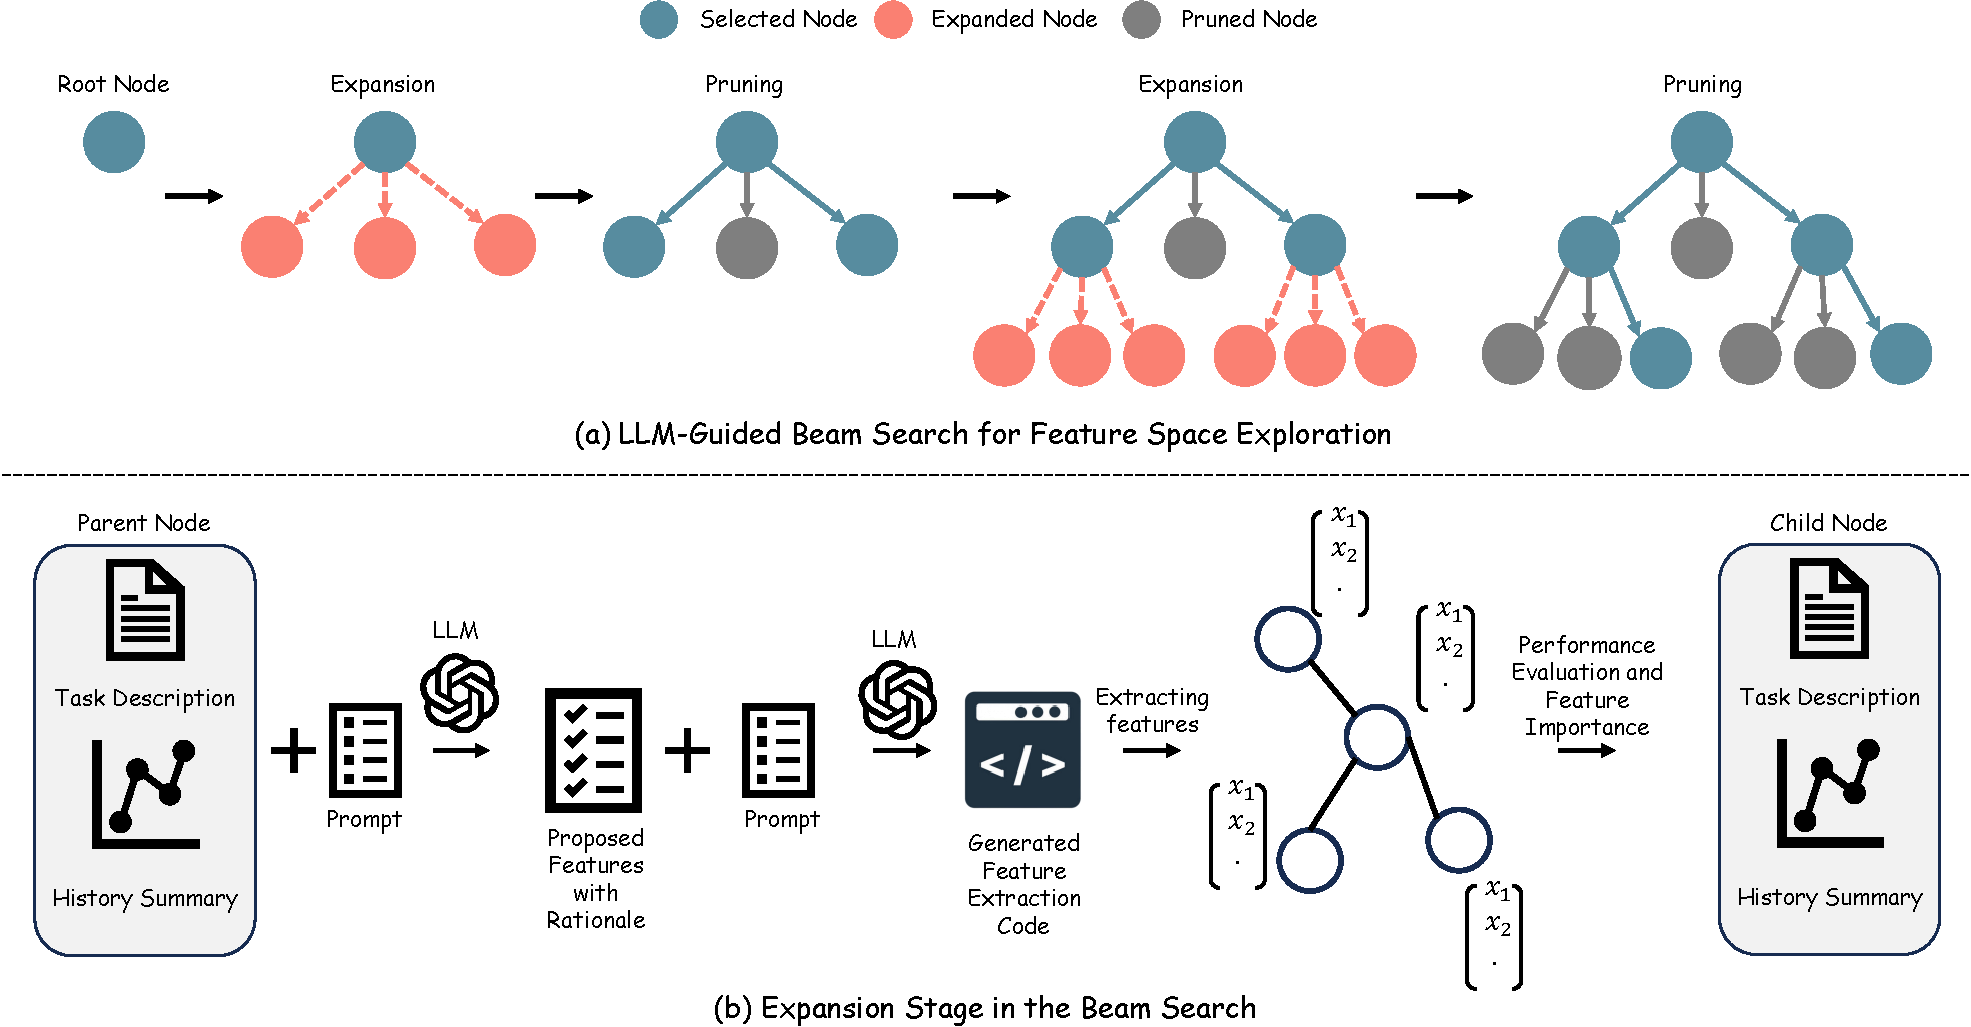
\includegraphics[width=0.95\textwidth]{figures/llm2prune/LLM_cropped.pdf}
  \caption{(a) Two phases of LLM2Prune, illustrated with beam width $\beta = 2$ and
    expansion factor $\gamma = 3$. In the expansion stage, each node expands into $\gamma$
    child nodes. In the pruning stage, the beam grows by another depth, keeping its width
    to $\beta$ after pruning out candidate nodes with poor performance. (b) An overview of
    the expansion stage. Each parent node, consisting of a task description and a history
    summary, is used to prompt the LLM to propose new features. A second prompt generates
    executable feature extraction code, which is applied to produce features. These are
    evaluated for performance and importance, and the resulting history is carried forward
    to form child nodes.}
  \label{fig:llm2prune-framework}
\end{figure}

\subsection{Decision Tree Formulation}

Each node $n_{d,i}$ in the decision tree (where $d$ indicates depth and $i$ indexes the
node at that depth) is represented as a tuple:
\[
n_{d,i} = \big(\mathcal{F}_{d,i}, \mathcal{M}_{d,i}, g_{\theta_{d,i}}, \mathcal{H}_{d,i}\big),
\]
where $\mathcal{F}_{d,i}$ is the proposed feature set, $g_{\theta_{d,i}}$ is the trained
classifier on $\mathcal{F}_{d,i}$, and $\mathcal{M}_{d,i}$ denotes the performance metric
of the classifier, defined as the combined metric $C = P_r \cdot P_g$ evaluated on a
held-out synthetic validation graph. The final component, $\mathcal{H}_{d,i}$, represents
the cumulative history, defined as the accumulation of all feature sets, performance
metrics, feature-importance vectors, and discarded features along the unique path from the
root node $n_{0,1}$ to node $n_{d,i}$:
\[
\mathcal{H}_{d,i} = \bigcup_{\ell=0}^{d} \bigcup_{j \in \pi(\ell,i)}
\Big(\mathcal{F}_{\ell,j}, M_{\ell,j}, \text{Imp}_{\ell,j}, \mathcal{F}^{\text{fail}}_{\ell,j}\Big),
\]
where $\pi(\ell,i)$ denotes the ancestor index at depth $\ell$ along the path from the
root to $n_{d,i}$, $M_{\ell,j}$ is the performance metric, $\text{Imp}_{\ell,j}$ is the
feature-importance vector, and $\mathcal{F}^{\text{fail}}_{\ell,j}$ is the set of features
discarded due to exceeding a timeout threshold. The cumulative history ensures that the LLM
generates new feature proposals with full awareness of the trajectory that led to the
current node. Conditioning on the full root-to-node path rather than only the immediate
parent prevents the LLM from re-proposing features explored and discarded at earlier
depths.

\subsection{Expansion Phase}

The algorithm expands the search tree one depth level at a time. At each depth $d$, for
each node $n_{d,i}$ in the current beam $B_d$, the expansion phase generates $\gamma$
child nodes through the following steps:

First, the LLM summarizes the cumulative history $\mathcal{H}_{d,i}$ using a summary
meta-prompt $Z_{\text{summary}}$, which condenses the feedback into key points and
insights. This keeps the feedback compact and makes the reasoning process easier for the
LLM to follow. Then, using a feature-generation meta-prompt $Z_{\text{feature}}$
conditioned on the task description with constraints and the history summary, the LLM
proposes $\gamma$ child feature sets. The meta-prompt provides higher-level guidance: it
instructs the LLM to enumerate and retain important features, remove redundant or
uninformative ones, and propose new features derived from the current set of
high-performing features. Formally, the child feature sets are sampled as:
\[
\big\{\mathcal{F}_{d+1,j}\big\}_{j=1}^{\gamma} \;\sim\;
\text{LLM}\big(Z_{\text{feature}}, \text{Task}, \text{Summary}(\mathcal{H}_{d,i})\big).
\]
A key property is that the LLM is stochastic: even under identical inputs, it can generate
diverse outputs due to sampling mechanisms such as temperature, thereby broadening
exploration of the feature space.

For each child node with its generated feature set $\mathcal{F}_{d+1,j}$, the LLM is
prompted with a code-generation meta-prompt $Z_{\text{code}}$ to produce executable Python
code for each proposed feature. Each feature must return a NumPy array with one value per
node. A timeout threshold $\tau$ is imposed to ensure computational efficiency: if
execution exceeds $\tau$, the failure is recorded in the history and the corresponding
feature is discarded. This mechanism keeps the pruning process lightweight by excluding
costly features and prevents further exploration of features correlated with discarded
ones.

A classifier $g_\theta$ (a two-layer GCN~\citep{kipf2016semi}) is then trained on the
features in $\mathcal{F}_{d+1,j}$ using semi-supervised learning. After a warm-up period,
the classifier retains high-confidence nodes:
\[
\mathcal{V}_{\text{conf}} = \{v \in \mathcal{V} : \max_y p_\theta(y \mid v) \geq \delta\},
\]
where $\delta$ is a confidence threshold. For each $v \in \mathcal{V}_{\text{conf}}$, soft
pseudo-labels $\tilde{y}_v = p_\theta(y \mid v)$ are assigned. These soft pseudo-labels,
together with the ground-truth labels on the supervised subset, guide further training and
improve robustness by incorporating uncertainty rather than enforcing hard assignments.
This approach mitigates label noise that arises when all non-solution nodes are treated as
equally unimportant~\citep{manchanda2020gcomb}.

Feature-importance scores are then extracted using
GNNExplainer~\citep{ying2019gnnexplainer}, which provides attribution scores indicating
each feature's contribution to the classifier's predictions. These scores form the
feedback signal $\text{Imp}_{d,i}$ used to guide subsequent feature generation.

\subsection{Pruning Phase}

After expanding all nodes at depth $d$, the algorithm evaluates each candidate child node
$n_{d+1,j}$ using its performance metric $M_{d+1,j}$ and constructs the next beam
$B_{d+1}$ by selecting the top-$\beta$ nodes:
\[
B_{d+1} \subseteq \mathcal{C}_{d+1}, \quad |B_{d+1}| = \beta.
\]
The process continues until the search reaches a maximum depth $D_{\max}$. At this point,
the best node across the entire tree is returned:
\[
n^{\text{best}} = \arg\max_{n_{d,i} \in \mathcal{T}} M_{d,i}.
\]
The classifier $g_{\theta^{\text{best}}}$ is then fine-tuned on the actual target training
graph and applied to prune the ground set $\mathcal{U}$. The beam search is performed once
on synthetic graphs that match the structural distribution of the target domain.
Algorithm~\ref{alg:llm2prune} describes the full LLM2Prune pipeline.

\begin{algorithm}[t]
\caption{LLM2Prune}
\label{alg:llm2prune}
\begin{algorithmic}[1]
\REQUIRE Task description, ground set $\mathcal{U}$, beam width $\beta$, expansion factor $\gamma$, max depth $D_{\max}$, timeout $\tau$, confidence threshold $\delta$
\ENSURE Pruned ground set $\mathcal{U}' \subseteq \mathcal{U}$
\STATE Initialize root node $n_{0,1}$ with empty feature set and history $\mathcal{H}_{0,1} = \emptyset$
\STATE $B_0 \leftarrow \{n_{0,1}\}$
\FOR{$d = 0, 1, \dots, D_{\max} - 1$}
    \STATE $\mathcal{C}_{d+1} \leftarrow \emptyset$
    \FOR{each $n_{d,i} \in B_d$}
        \STATE $\text{summary} \leftarrow \text{LLM}(Z_{\text{summary}}, \mathcal{H}_{d,i})$
        \FOR{$j = 1, \dots, \gamma$}
            \STATE $\mathcal{F}_{d+1,j} \sim \text{LLM}(Z_{\text{feature}}, \text{Task}, \text{summary})$
            \STATE Generate and execute code for each $f \in \mathcal{F}_{d+1,j}$; discard features exceeding $\tau$
            \STATE Train $g_{\theta_{d+1,j}}$ on $\mathcal{F}_{d+1,j}$ with semi-supervised learning (threshold $\delta$)
            \STATE Compute $M_{d+1,j}$ and $\text{Imp}_{d+1,j}$; update $\mathcal{H}_{d+1,j}$
            \STATE $\mathcal{C}_{d+1} \leftarrow \mathcal{C}_{d+1} \cup \{n_{d+1,j}\}$
        \ENDFOR
    \ENDFOR
    \STATE $B_{d+1} \leftarrow \text{top-}\beta$ nodes in $\mathcal{C}_{d+1}$ by $M$ \hfill \textit{// Beam Pruning}
\ENDFOR
\STATE $n^{\text{best}} \leftarrow \arg\max_{n_{d,i} \in \mathcal{T}} M_{d,i}$
\STATE Fine-tune $g_{\theta^{\text{best}}}$ on the target training graph
\RETURN top-ranked nodes of $\mathcal{U}$ under $g_{\theta^{\text{best}}}$ as $\mathcal{U}'$
\end{algorithmic}
\end{algorithm}

\section{Preliminary Results}

We have conducted preliminary experiments to validate the proposed approach. We evaluate
LLM2Prune on three graph CO problems, namely Maximum Coverage (MaxCover), Maximum Cut
(MaxCut), and Influence Maximization (IM), under both size and knapsack constraints, using
eight real-world datasets from the Stanford Large Network Dataset
Collection~\citep{leskovec2016snap}. The same datasets and train-test splits as in
Chapters~3 and~4 are used, following~\citep{ireland2022lense}. For size constraints,
Standard Greedy~\citep{nemhauser1978analysis} is used for MaxCover and MaxCut, and
IMM~\citep{tang2015influence} for IM. Under knapsack constraints,
\citet{khuller1999budgeted} is used for IM and MaxCover, and \citet{pham2023linear} for
MaxCut. The cost of each node under knapsack constraints is set proportional to its degree
following~\citep{pmlr-v258-nath25a, yaroslavtsev2020bring}. Since running beam search on
each instance would be costly, we perform feature-space search using the Holme-Kim random
graph model~\citep{holme2002growing}, which closely resembles large-scale social networks
with both scale-free degree distribution and high clustering coefficient. After identifying
the feature set, we fine-tune the downstream classifier for each instance.

\subsection{Size Constraint Results}

Under the size constraint, we compare LLM2Prune with classical methods
(QuickPrune~\citep{pmlr-v258-nath25a} and Submodular
Sparsification~\citep{zhou2017scaling}) and learning-based methods
(GCOMB-P~\citep{manchanda2020gcomb}, LeNSE~\citep{ireland2022lense}, and
COMBHelper~\citep{tian2024combhelper}). Table~\ref{tab:llm2prune-size} reports the results
for Maximum Cut and Influence Maximization.

\begin{table}[t]
\centering
\caption{Comparison of pruning algorithms under size constraints. Reported are the pruning
  approximation ratio ($P_r$), pruned fraction ($P_g$), and combined metric ($C = P_r
  \cdot P_g$). Results for GCOMB-P, LeNSE, and COMBHelper are reported
  from~\citep{ireland2022lense, pmlr-v258-nath25a}. ``--'' indicates no reasonable result.}
\label{tab:llm2prune-size}
\resizebox{\textwidth}{!}{%
\begin{tabular}{lccc|ccc|ccc|ccc|ccc|ccc}
\toprule
 & \multicolumn{6}{c}{\textbf{Classical Approach}} & \multicolumn{12}{c}{\textbf{Learning-Based Approach}} \\
\cmidrule(lr){2-7} \cmidrule(lr){8-19}
 \textbf{Dataset} & \multicolumn{3}{c}{\textsc{QuickPrune}} & \multicolumn{3}{c}{SS} & \multicolumn{3}{c}{\textbf{LLM2Prune}} & \multicolumn{3}{c}{GCOMB-P} & \multicolumn{3}{c}{\textsc{LeNSE}} & \multicolumn{3}{c}{\textsc{COMBHelper}} \\
& $P_r$ & $P_g$ & $C$ & $P_r$ & $P_g$ & $C$ & $P_r$ & $P_g$ & $C$ & $P_r$ & $P_g$ & $C$ & $P_r$ & $P_g$ & $C$ & $P_r$ & $P_g$ & $C$ \\
\midrule
\multicolumn{19}{c}{\textbf{Maximum Cut}} \\
\midrule
Facebook & 0.9886 & 0.7935 & 0.7845 & 0.9928 & 0.9027 & 0.8962 & 1.0004 & 0.7501 & 0.7504 & 0.8130 & 0.9500 & 0.7723 & 1.0000 & 0.0700 & 0.0700 & 1.0000 & 0.1538 & 0.1538 \\
DBLP & 1.0000 & 0.9954 & 0.9954 & 1.0000 & 0.9963 & 0.9963 & 0.9981 & 0.9841 & 0.9822 & 0.6460 & 0.9900 & 0.6395 & 0.9930 & 0.9200 & 0.9136 & 1.0000 & 0.1825 & 0.1825 \\
Deezer & 0.9996 & 0.9730 & 0.9726 & 0.9999 & 0.9855 & 0.9854 & 0.9999 & 0.9907 & 0.9906 & 0.8500 & 0.9900 & 0.8415 & 0.9750 & 0.7400 & 0.7215 & 1.0000 & 0.3754 & 0.3754 \\
Slashdot & 1.0000 & 0.9904 & 0.9904 & 1.0000 & 0.9889 & 0.9889 & 1.0000 & 0.9926 & 0.9926 & 0.6320 & 0.9900 & 0.6257 & 0.9900 & 0.6200 & 0.6138 & 0.7935 & 0.9929 & 0.7879 \\
Wiki & 0.9985 & 0.9037 & 0.9023 & 0.9981 & 0.9346 & 0.9328 & 1.0000 & 0.9214 & 0.9214 & 0.9200 & 0.9600 & 0.8832 & 0.9810 & 0.3900 & 0.3826 & 1.0000 & 0.7011 & 0.7011 \\
Twitter & 1.0000 & 0.9900 & 0.9900 & 1.0000 & 0.9893 & 0.9893 & 1.0000 & 0.9938 & 0.9938 & 0.6280 & 0.9900 & 0.6217 & 0.9870 & 0.4800 & 0.4738 & 1.0000 & 0.5542 & 0.5542 \\
YouTube & 1.0000 & 0.9994 & 0.9994 & 1.0000 & 0.9987 & 0.9987 & 1.0000 & 0.9991 & 0.9991 & 0.5360 & 0.9900 & 0.5306 & 0.9870 & 0.7900 & 0.7797 & 0.9990 & 0.9705 & 0.9695 \\
Skitter & 1.0000 & 0.9995 & 0.9995 & 1.0000 & 0.9991 & 0.9991 & 0.9966 & 0.9988 & 0.9954 & 0.4270 & 0.9900 & 0.4227 & 0.9740 & 0.7100 & 0.6915 & -- & -- & -- \\
\midrule
\multicolumn{19}{c}{\textbf{Influence Maximization}} \\
\midrule
Facebook & 0.9919 & 0.7450 & 0.7390 & 0.9208 & 0.9027 & 0.8312 & 0.9995 & 0.7501 & 0.7498 & 0.9510 & 0.7300 & 0.6942 & 0.9790 & 0.0900 & 0.0881 & 1.0039 & 0.3248 & 0.3261 \\
DBLP & 0.8603 & 0.9946 & 0.8557 & 1.0495 & 0.9963 & 1.0456 & 0.9953 & 0.9984 & 0.9937 & 0.8630 & 0.9900 & 0.8544 & 0.9690 & 0.8900 & 0.8624 & 0.9873 & 0.0194 & 0.0192 \\
Deezer & 0.9384 & 0.9698 & 0.9101 & 1.0262 & 0.9855 & 1.0113 & 0.9759 & 0.9907 & 0.9668 & 0.8050 & 0.5500 & 0.4428 & 0.9720 & 0.7600 & 0.7387 & 0.9837 & 0.1093 & 0.1075 \\
Slashdot & 0.9984 & 0.9881 & 0.9865 & 0.9959 & 0.9889 & 0.9848 & 1.0215 & 0.9926 & 1.0139 & 0.9660 & 0.9800 & 0.9467 & 0.9660 & 0.7700 & 0.7438 & 1.0076 & 0.9875 & 0.9950 \\
Wiki & 1.0269 & 0.8831 & 0.9069 & 0.9863 & 0.9346 & 0.9218 & 1.0039 & 0.9214 & 0.9249 & 0.9690 & 0.9000 & 0.8721 & 0.9600 & 0.5100 & 0.4896 & 0.9969 & 0.6066 & 0.6047 \\
Twitter & 1.0045 & 0.9965 & 1.0010 & 0.9575 & 0.9893 & 0.9473 & 0.9817 & 0.9876 & 0.9695 & 0.9200 & 0.9800 & 0.9016 & 0.9660 & 0.4000 & 0.3864 & 0.9972 & 0.4947 & 0.4933 \\
YouTube & 0.9677 & 0.9994 & 0.9671 & 0.9846 & 0.9987 & 0.9833 & 1.0005 & 0.9991 & 0.9996 & 0.9330 & 0.9900 & 0.9237 & 0.9710 & 0.7500 & 0.7282 & 0.9992 & 0.9705 & 0.9697 \\
Skitter & 0.9813 & 0.9999 & 0.9812 & 1.0032 & 0.9991 & 1.0023 & 1.0035 & 0.9970 & 1.0006 & 0.8830 & 0.9900 & 0.8742 & 0.9830 & 0.7800 & 0.7667 & -- & -- & -- \\
\bottomrule
\end{tabular}
}
\end{table}

From Table~\ref{tab:llm2prune-size}, LLM2Prune performs competitively with classical
methods such as QuickPrune and SS on the combined metric. However, both classical
approaches rely on sequential submodularity-based pruning, which is orders of magnitude
slower than LLM2Prune on large datasets such as YouTube and Skitter
(Figure~\ref{fig:llm2prune-runtime}). In contrast, LLM2Prune achieves comparable or
better performance without relying on hand-crafted features, demonstrating that
learning-based pruning can be both effective and efficient. Within the learning-based
category, LLM2Prune outperforms prior methods in both combined metric and runtime.
GCOMB-P and COMBHelper frequently underperform, while LeNSE is more stable but generally
results in lower combined-metric values. Unlike other learning-based methods that depend
on handcrafted features, LLM2Prune balances efficiency with strong performance,
effectively narrowing the gap with classical methods.

\begin{figure}[t]
  \centering
  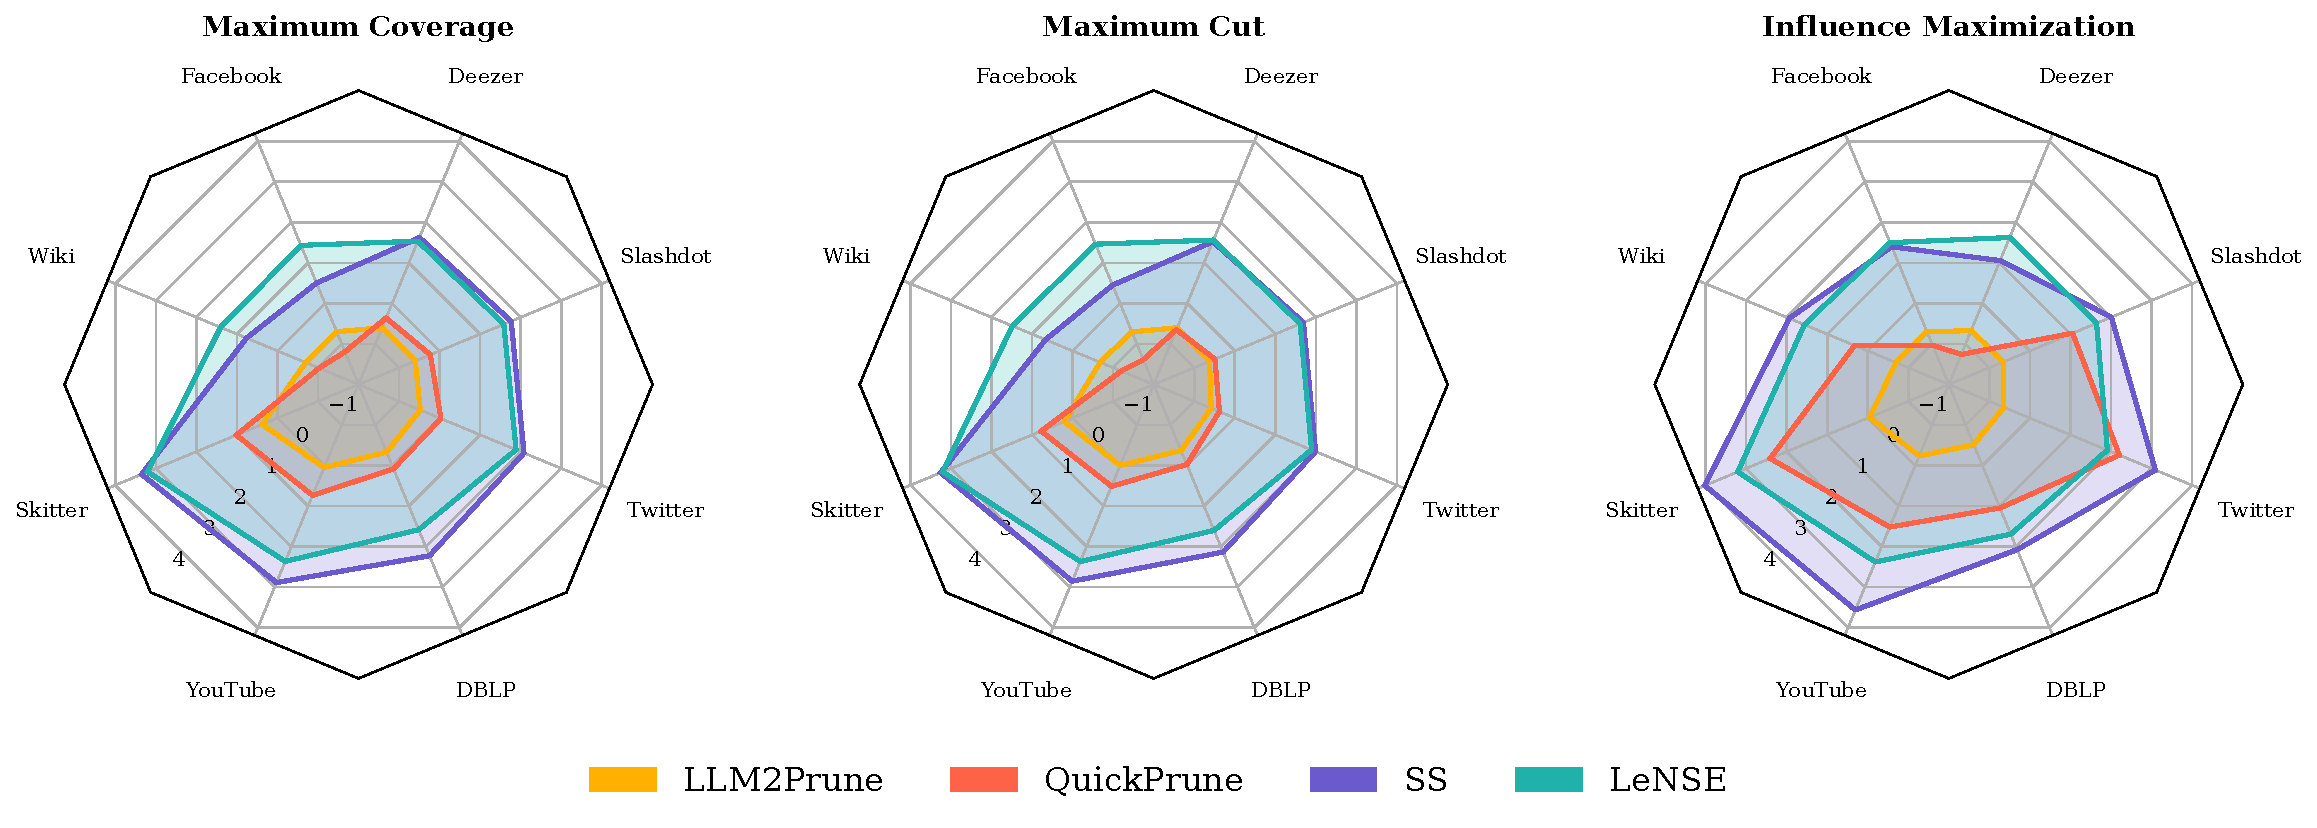
\includegraphics[width=0.9\textwidth]{figures/llm2prune/runtimes_radar.pdf}
  \caption{Runtime comparison (log scale) of pruning algorithms on Maximum Coverage,
    Maximum Cut, and Influence Maximization across eight datasets.}
  \label{fig:llm2prune-runtime}
\end{figure}

\subsection{Discovered Features}

A key strength of LLM2Prune is that it generates features that are not generic graph
statistics but are grounded in the problem objective. For MaxCut, it discovers \emph{random
cut expectation}, the expected marginal contribution of a node to the cut under a random
partition, a non-trivial descriptor directly derived from the cut objective. For IM, it
identifies \emph{average incoming activation probability} and \emph{outgoing activation
probability sum}, which require reasoning about the independent cascade model and capture a
node's susceptibility and direct influence spread, respectively. These features would
require significant domain expertise to design manually, yet LLM2Prune discovers them
automatically from the task description alone.

\subsection{Ablation Study}

To justify the choice of beam search, we conducted an ablation study comparing four
variants using the same number of API calls: (1)~a single-shot prompt with no iterative
refinement, (2)~a simple feedback loop with performance metrics only, (3)~a simple feedback
loop with both performance metrics and feature-importance scores, and (4)~the full beam
search. Figure~\ref{fig:llm2prune-ablation} reports the combined metric across three CO
problems. The results show that beam search consistently achieves higher and more stable
performance, with median values close to $1.0$ and minimal variance across runs. Simpler
variants suffer from error propagation when early iterations contain reasoning errors,
whereas beam search mitigates this issue by maintaining multiple candidate paths.

\begin{figure}[t]
  \centering
  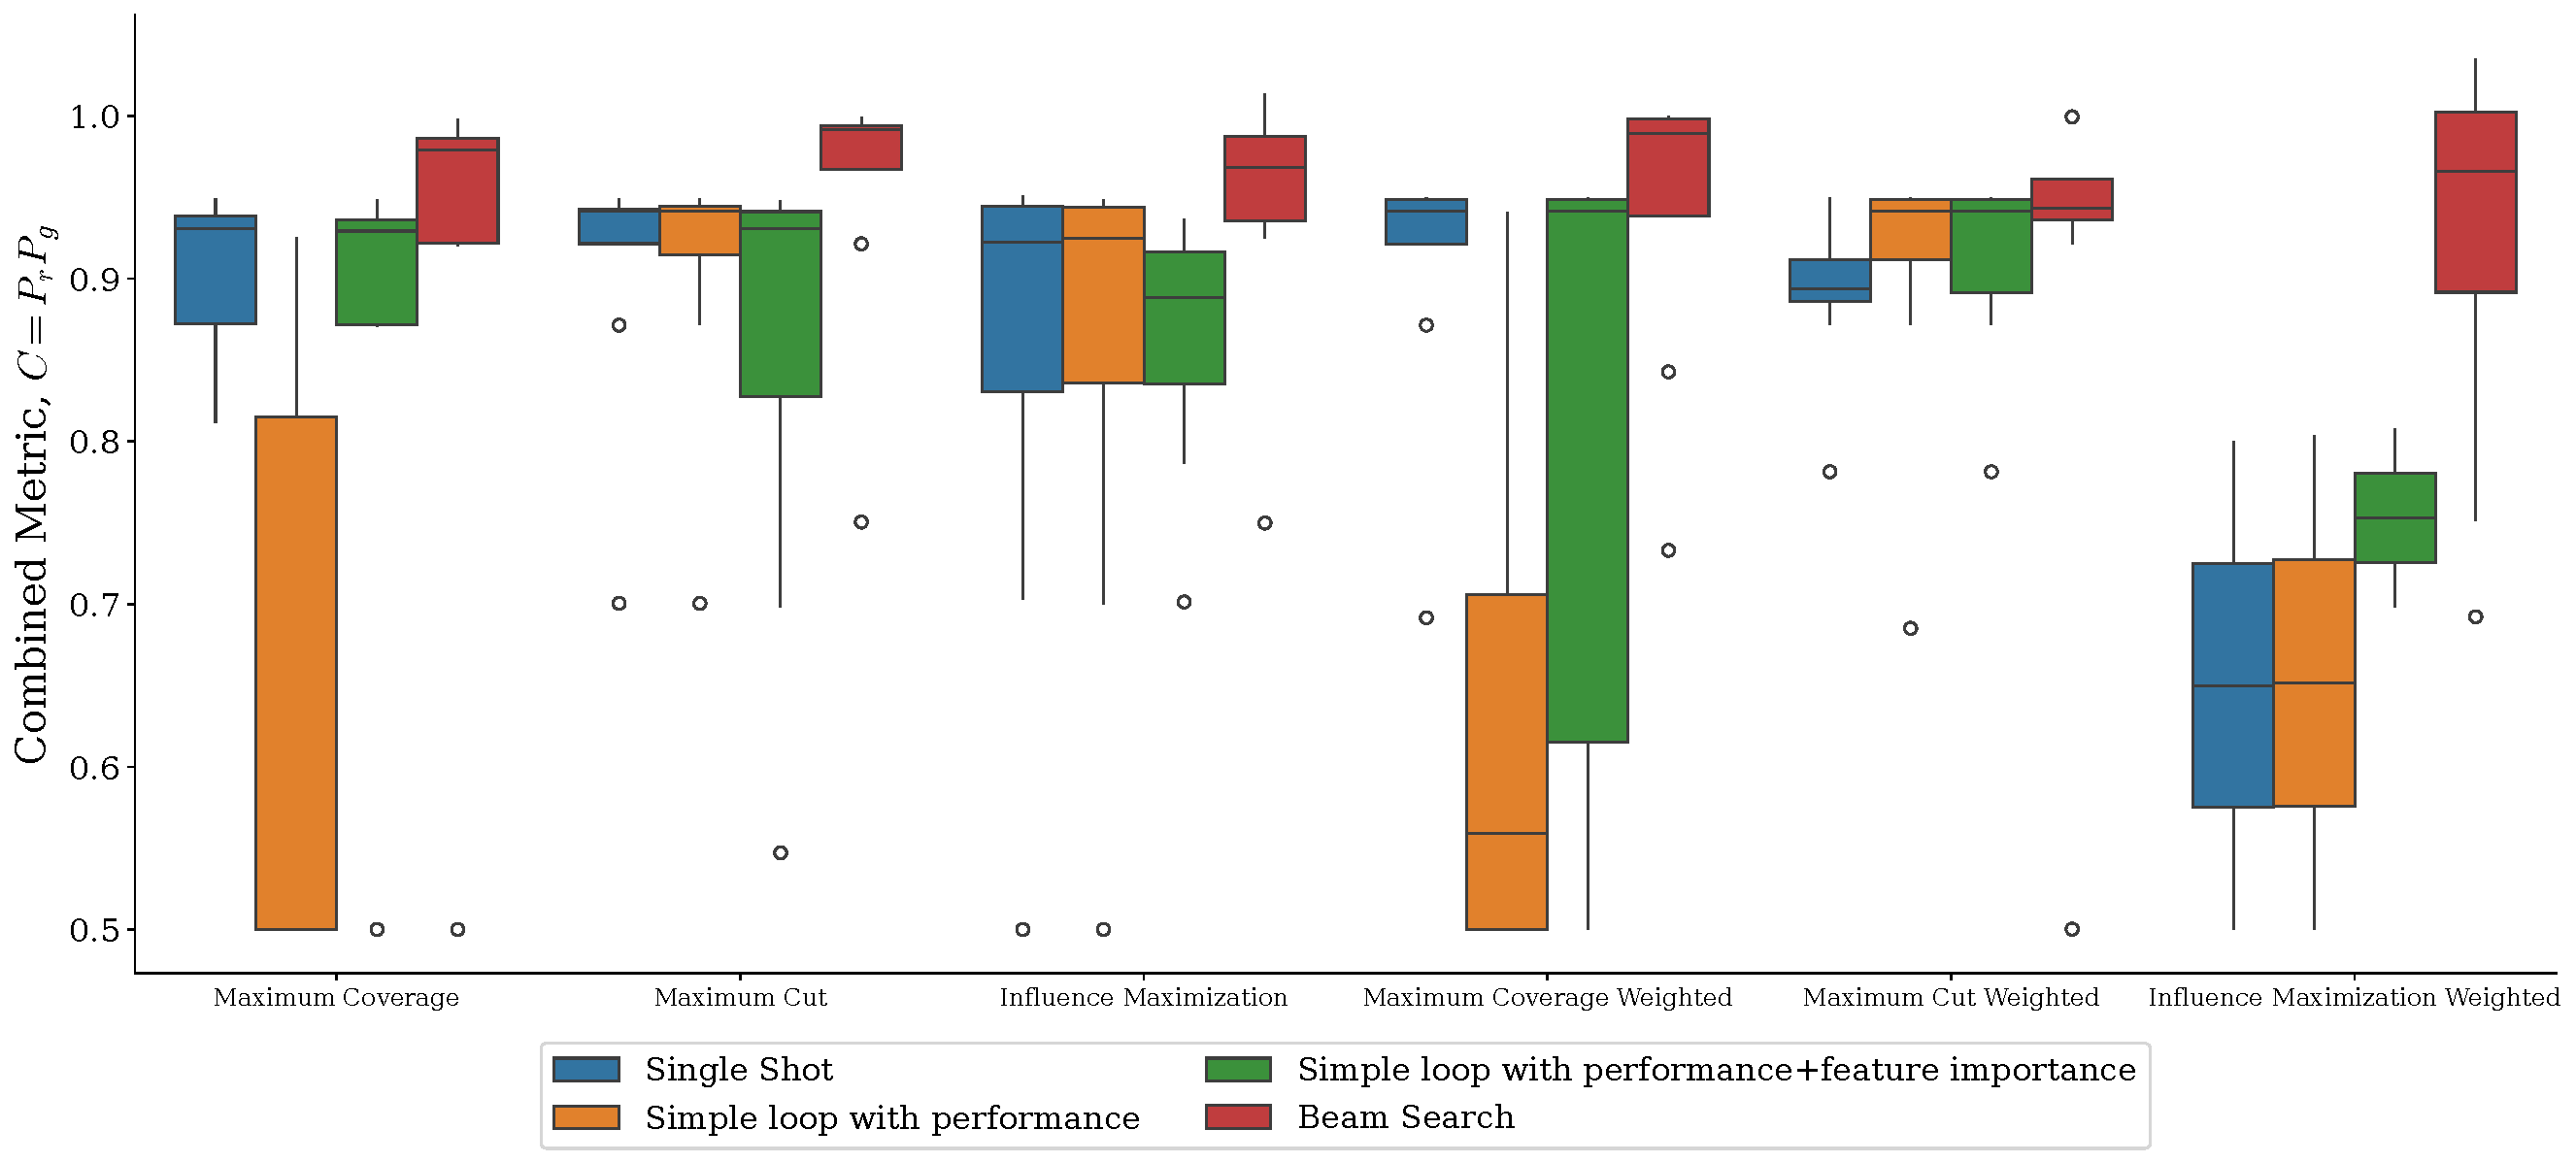
\includegraphics[width=\textwidth]{figures/llm2prune/ablation.pdf}
  \caption{Performance comparison of different variants of LLM2Prune. Beam search achieves
    higher and more stable performance compared to single-shot and simple feedback loop
    variants.}
  \label{fig:llm2prune-ablation}
\end{figure}

\section{Remaining Work}

We have completed the proposed framework design, the ablation study justifying the beam
search strategy, and a comprehensive evaluation under size constraints across three CO
problems and eight real-world datasets. The results demonstrate that LLM2Prune performs
competitively with classical methods while being orders of magnitude faster at inference,
and consistently outperforms all existing learning-based approaches. The primary remaining
work is to conduct a comprehensive evaluation under knapsack constraints across all
datasets and applications. Unlike other learning-based methods, LLM2Prune can naturally
adapt to the knapsack constraint by simply modifying the task description provided to the
LLM, without requiring any changes to the underlying framework or retraining the feature
discovery pipeline.
